\spacing{1.3}
\renewcommand{\tablename}{Tabla}


%\section{Organización de la Tabla Periódica (TP) de los elementos}\label{sec:organizacion-de-la-tabla-periodica-(tp)-de-los-elementos}
%
%A partir del siglo XIX, la clasificación de los elementos químicos conocidos hasta el momento se convirtió en una necesidad.
%
%\subsection{Primeros intentos de clasificación}\label{subsec:primeros-intentos-de-clasificacion}
%
%\begin{enumerate}
%    \item \textbf{Distinción entre metales y no metales}.
%    \item \textbf{Triadas de Döbereiner}.
%    Consistía en agrupar los elementos de tres en tres de tal forma que la masa atómica del segundo constituyese aproximadamente la media de las masas atómicas de los otros dos, además, las propiedades químicas del elemento central eran intermedias con respecto a las de los otros dos.
%    \item \textbf{Octavas de Newlands}.
%    Disponía los elementos químicos por orden creciente de su masa atómica, resultaba que cada siete elementos se repetía la secuencia de propiedades.
%    \item \textbf{Tabla de Mendeléyev y Meyer}.
%    Trabajando de manera independiente, basaron la clasificación en la ordenación de los elementos según un orden creciente de su masa atómica teniendo en cuenta las propiedades físicas y químicas agrupándolos en la misma columna o grupo.
%\end{enumerate}

\section{Tabla periódica (TP) actual}\label{subsec:tabla-periodica-(tp)-actual}

En la TP actual, los elementos se ordenan según el orden creciente de su número atómico, y esta muestra cómo se repiten las propiedades químicas y físicas.
La TP está organizada en:
\begin{enumerate}[label=\numberballmDarkTeal]
        \item \textbf{Periodos}: son las filas de la TP y están formados por todos los elementos que tienen el mismo nivel energético superior ocupado, es decir, el mismo número cuántico $\bm{n}$ mayor con \el{}.
        \item \textbf{Grupos}: son las columnas y están formadas por elementos que presentan una configuración electrónica similar en su nivel más alto.
\end{enumerate}

Los nombres de los grupos y la configuración electrónica (siendo \(n\) el último nivel ocupado por los electrones) de su capa de valencia son:

\begin{itemize}
    \item \textbf{Grupo 1: Alcalinos}: $ns^1$
    \item \textbf{Grupo 2: Alcalinotérreos}: $ns^2$
    \item \textbf{Grupo 3: Metales de transición} $ns^2(n-1)d^1$
    \item \textbf{Grupo 4: Metales de transición} $ns^2(n-1)d^2$
    \item \textbf{Grupo 5: Metales de transición} $ns^2(n-1)d^3$
    \item \textbf{Grupo 6: Metales de transición} $ns^2(n-1)d^4$
    \item \textbf{Grupo 7: Metales de transición} $ns^2(n-1)d^5$
    \item \textbf{Grupo 8: Metales de transición} $ns^2(n-1)d^6$
    \item \textbf{Grupo 9: Metales de transición} $ns^2(n-1)d^7$
    \item \textbf{Grupo 10: Metales de transición} $ns^2(n-1)d^8$
    \item \textbf{Grupo 11: Metales de transición} $ns^2(n-1)d^9$
    \item \textbf{Grupo 12: Metales de transición} $ns^2(n-1)d^{10}$
    \item \textbf{Grupo 13: Boroideos} $ns^2np^1$
    \item \textbf{Grupo 14: Carbonoideos} $ns^2np^2$
    \item \textbf{Grupo 15: Nitrogenoideos} $ns^2np^3$
    \item \textbf{Grupo 16: Anfígenos} $ns^2np^4$
    \item \textbf{Grupo 17: Halógenos} $ns^2np^5$
    \item \textbf{Grupo 18: Gases nobles} $ns^2np^6$
    \item \textbf{Elementos de transición interna o grupo $f$} $ns^2(n-2)f^1 \longrightarrow ns^2(n-2)f^{14}$
\end{itemize}
Al final de la unidad, en Figura \ref{fig:tp} tenéis una tabla periódica.
% \newpage
% \begin{landscape}

%     \begin{figure}[H]
%         \centering
%         \includegraphics[scale=0.5]{images/UD2/tp.png}
%         \caption{Tabla Periódica}
%         \label{fig:tp}
%     \end{figure}

% \begin{figure}[H]
%     \centering
%     \includegraphics[scale=0.6]{tp.png}
%     \caption{Tabla periódica}
%     \label{fig:tp}
%\end{figure}

% \end{landscape}


\section{Propiedades Periódicas}\label{sec:propiedades-periodicas}

Las propiedades periódicas son propiedades de los elementos químicos cuyo valor se puede prever de manera cualitativa observando la posición que ocupan en la tabla periódica.
Su valor depende de:
\begin{enumerate}[label=\numberballmDarkTeal]
        \item \negrita{Carga nuclear (\( Z \))}: nos dice cómo de atraídos están los electrones por el núcleo. A mayor carga nuclear, mayor atracción. Por norma general, al aumentar el número atómico, aumenta la carga nuclear.
        \begin{remark}
            Aunque la carga nuclear y el número atómico se representan con la misma letra, no deben confundirse.
        \end{remark}
%         se trata de la carga positiva del núcleo del átomo.
%        La carga nuclear nos dice cómo están atraídos los electrones por el núcleo.
%        Podemos decir que al aumentar el número atómico \(Z\) también aumentará la carga nuclear debido a que tenemos más protones y, por tanto, aumenta la carga positiva.
%        A mayor valor de la carga nuclear mayor atracción de los electrones por el núcleo.
%        Es importante no confundir la carga nuclear con el número atómico.
        \item \negrita{Efecto pantalla (\( \sigma \))}: es la interacción que tienen los electrones de las diferentes capas que hace que se repelan unos con otros. Este apantallamiento hace que la carga nuclear disminuya.
        \begin{figure}[H]
            \centering
            % [FIGURA ORIGINAL] \includegraphics[scale=.5]{images/imagesUD2TablaPeriodica/UD2_Teoria/apantallamientod}
            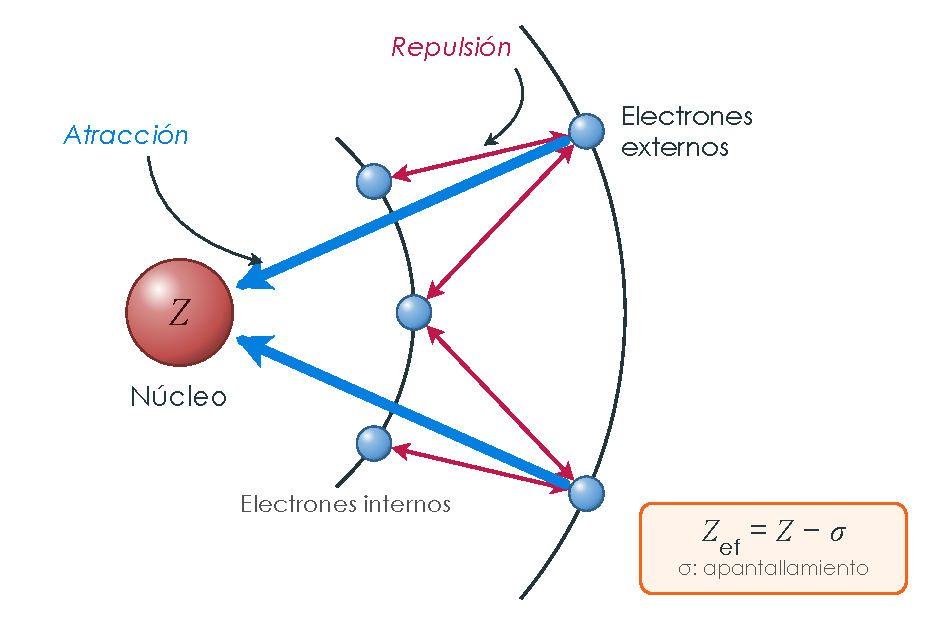
\includegraphics[width=0.65\linewidth]{FigurasSVG/UD2_Tabla_Periodica/pdf/UD2_01_apantallamiento.pdf}
            \caption{Apantallamiento de electrones}
            \label{fig:apantallamiento}
        \end{figure}
        El efecto pantalla no tiene sentido estimarlo entre los elementos de un mismo período porque todos los elementos tienen ocupado el mismo nivel energético.
        El efecto pantalla sí tiene sentido estudiarlo entre los elementos de un mismo grupo, ya que al ir bajando en el grupo, aumentarán los niveles energéticos llenados y, por tanto, el apantallamiento es mayor.
        \item \negrita{Capa de valencia}: capa en la que se encuentran los electrones más externos de un átomo.
        \item \negrita{Carga nuclear efectiva (\(\bm{Z_{eff}}\))}: es la carga nuclear teniendo en cuenta el apantallamiento y hace referencia a cómo los electrones están atraídos por el núcleo. Al $\uparrow\;Z_{eff}$ los electrones estarán más atraídos, mientras que si $\downarrow\;Z_{eff}$ los electrones estarán menos atraídos por el núcleo.
        La carga nuclear efectiva puede calcularse según la ecuación:
        \begin{centeredequation}
            Z_{eff} = Z - \sigma
        \end{centeredequation}

\end{enumerate}

\subsection{Radio atómico}\label{subsec:radio-atomico}

\begin{center}
    \begin{definition}[Radio atómico]
        Se puede definir como la distancia que separa el núcleo del átomo de su electrón más periférico.
        También lo podemos definir como la mitad de la distancia entre dos núcleos de átomos idénticos.
    \end{definition}
\end{center}

La variación del radio atómico está justificada por los siguientes factores:

\begin{enumerate}[label=\numberballmDarkTeal]
        \item Al aumentar la \textbf{carga nuclear}, el radio atómico tiende a ser menor, ya que aumenta la atracción electrostática del núcleo sobre la nube electrónica y hace que esta se aproxime más.
        Es el efecto más notorio en un período.
        \item Al descender en un grupo, aumenta el \textbf{efecto pantalla} y el radio atómico también aumenta.
        Al incrementarse el número de capas, aumenta la repulsión entre los electrones (aumenta el apantallamiento), por lo que su carga nuclear efectiva es menor y la nube electrónica se expande.
        Esto quiere decir que al bajar en un grupo hay más niveles energéticos con electrones, estos se repelen entre sí y, por tanto, se atraen menos por el núcleo, aumentando así el radio atómico.
        \item Al aumentar la \textbf{capa de valencia}, el radio atómico es \textbf{mayor}.
        La capa de valencia aumenta al descender en un grupo y no varía dentro de un período.
\end{enumerate}
% \begin{enumerate}[label=\numberballmDarkTeal]
%     \item \negrita{Grupo}: los radios atómicos crecen al aumentar el número atómico (al bajar en el grupo) y se debe a:
%     \begin{enumerate}
%         \item Al aumentar $Z$ tendremos un mayor número de electrones y por tanto el apantallamiento será mayor por lo que su $Z_{eff}$ será menor (los electrones menos atraídos por el núcleo).
%         \item Al bajar en el grupo aumentamos también el número de niveles y por lo tanto los electrones se encontrarán más alejados del número.
%     \end{enumerate}
%     \item \negrita{Periodo}: al ir de izquierda a derecha la carga nuclear irá aumentando y por lo tanto habrá más electrones que estarán mas atraídos por el núcleo disminuyendo así su radio. Aquí no tenemos en cuenta el apantallamiento porque al tener todos los mismos números de niveles energéticos el apantallamiento es similar.
% \end{enumerate}
Podemos decir que el radio atómico aumenta al descender en un grupo y al desplazarnos a la izquierda en un período, a excepción de los gases nobles.
Es decir, un átomo será tanto mayor cuanto más bajo y a la izquierda en la tabla periódica se encuentre el elemento correspondiente.
\begin{figure}[H]
    \centering
    % [FIGURA ORIGINAL] \includegraphics[scale=0.2]{images/imagesUD2TablaPeriodica/UD2_Teoria/variacionradio4}
    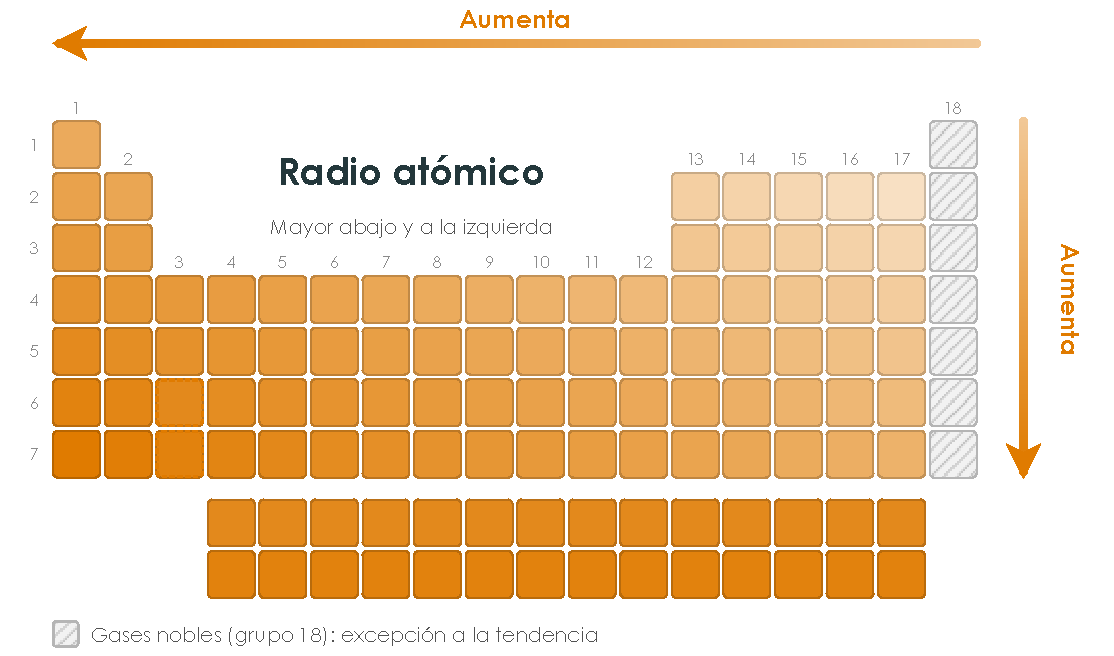
\includegraphics[width=0.85\linewidth]{FigurasSVG/UD2_Tabla_Periodica/pdf/UD2_02_variacion_radio_atomico.pdf}
    \caption{Variación del radio}
    \label{fig:variacionradio3}
\end{figure}

\subsubsection{Radio atómico en iones}

\begin{enumerate}[label=\numberballmDarkTeal]
        \item \negrita{Cationes}: tendrán siempre un radio \textbf{menor} que los elementos neutros, debido a que al perder un electrón, la atracción por el núcleo será mayor y, por tanto, disminuirá el radio.
        \item \negrita{Aniones}: tienen un radio \textbf{mayor} que los elementos neutros, ya que al aumentar el número de electrones, aumentará la repulsión disminuyendo así la atracción de los electrones por el núcleo.
\end{enumerate}
\begin{figure}[H]
    \centering
    % [FIGURA ORIGINAL] \includegraphics[scale=0.75]{images/imagesUD2TablaPeriodica/UD2_Teoria/variacioncationesaniones}
    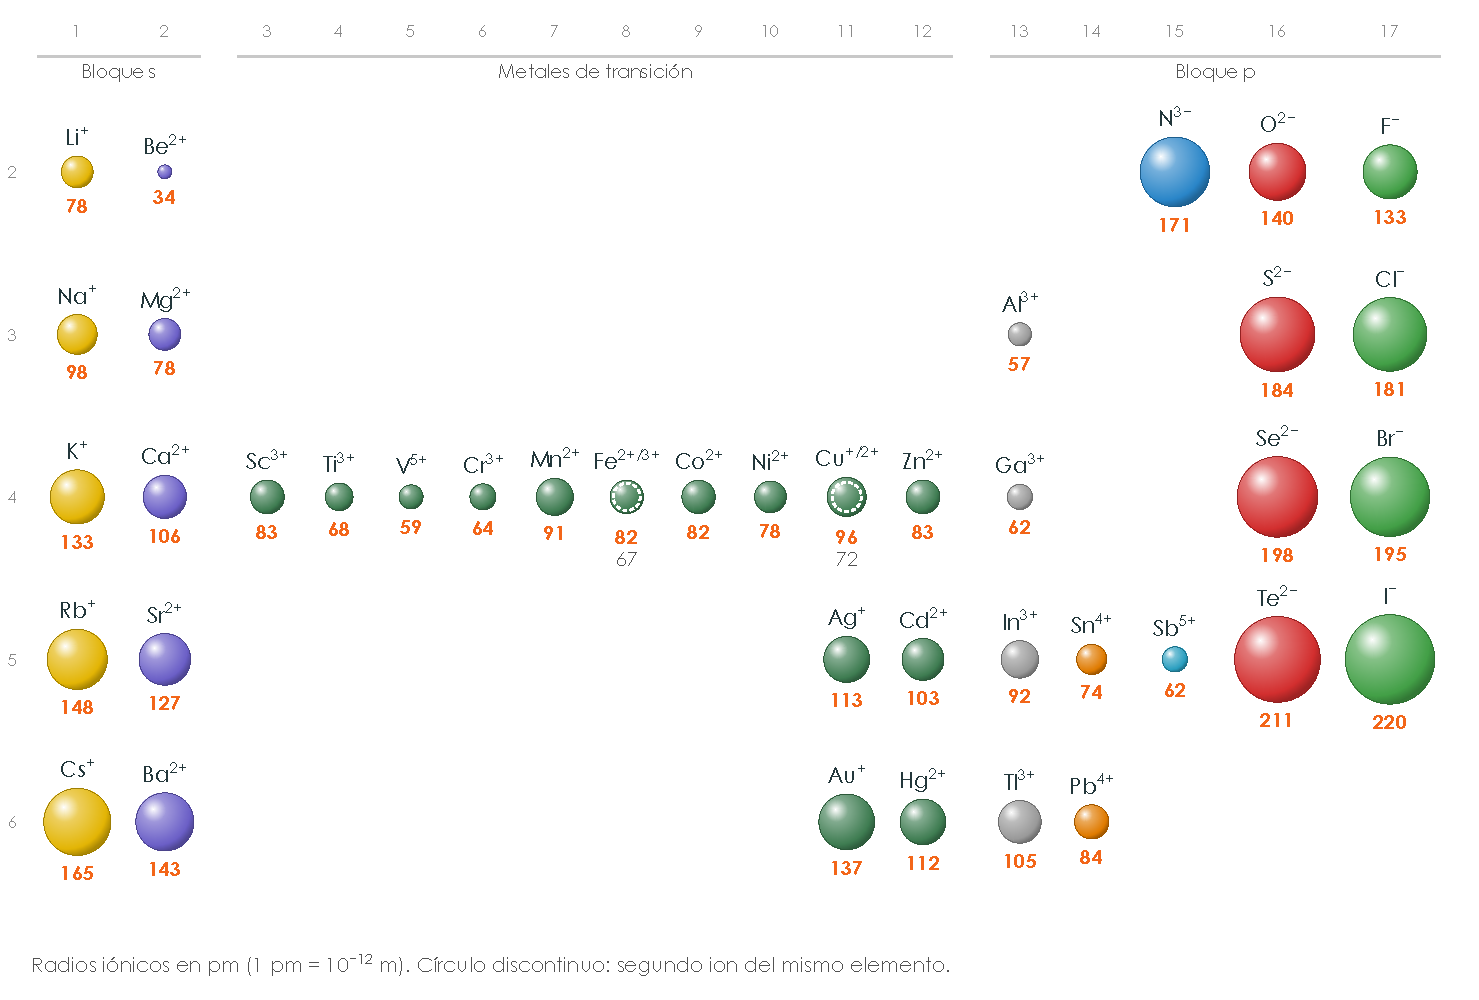
\includegraphics[width=1.0\linewidth]{FigurasSVG/UD2_Tabla_Periodica/pdf/UD2_03_radios_ionicos.pdf}
    \caption{Variación de cationes y aniones}
    \label{fig:variacioncationes}
\end{figure}

\subsection{Energía de ionización o potencial de ionización}\label{subsec:energia-de-ionizacion-o-potencial-de-ionizacion}


\begin{definition}[Energía de ionización (EI) o potencial de ionización (PI)]
        Es la energía necesaria para arrancar un electrón a un átomo en estado gaseoso.
        \begin{centeredequation}
             X(g)\longrightarrow X^+ (g) + e^-
        \end{centeredequation}
        Se mide en unidades de energía: \unit{\kilo\joule\per\mole}, \unit{\joule\per \text{átomo}}, \unit{\electronvolt\per \text{átomo}}.
\end{definition}

Los valores de las energías de ionización tienen signos positivos debido a que hay que administrar energía para provocar la eliminación de un electrón.

El primer electrón que se arranca es más fácil de extraer que el segundo y así sucesivamente, por lo que sus potenciales o energías de ionización van aumentando porque los electrones están cada vez más atraídos por el núcleo (1º PI \(<\) 2º PI \(<\) 3º PI ...).

La variación de la EI se justifica según los siguientes factores:

\begin{enumerate}[label=\numberballmDarkTeal]
        \item El potencial de ionización será mayor al aumentar la carga nuclear efectiva, puesto que los electrones están más atraídos por el núcleo.
        \item Al descender en un grupo, se intensifica el \textbf{efecto pantalla}, lo que provoca que disminuya la carga nuclear efectiva, disminuyendo así el potencial de ionización.
        \item Al avanzar en un período, aumenta la \textbf{carga nuclear}, aumentando así la atracción de los electrones por el núcleo, siendo más difícil extraer un electrón, lo que implica un mayor potencial de ionización.
        \item Al aumentar la capa de valencia (bajamos en un grupo), los electrones están más alejados del núcleo y, por ello, se necesita menos energía para arrancarlos.
\end{enumerate}
% \begin{enumerate}[label=\numberballmDarkTeal]
%     \item \negrita{Grupo}: al bajar en un grupo disminuye su EI ya que la carga nuclear efectiva será menor al ser el apantallamiento mayor y por tanto los electrones están menos atraídos por el núcleo.
%     \item \negrita{Periodo}: al ir de izquierda a derecha, la carga nuclear aumenta por lo que los electrones están más atraídos por el núcleo y por tanto su EI de ionización será mayor.
% \end{enumerate}

Podemos decir que el potencial de ionización aumenta al subir en un grupo y al desplazarse a la derecha del período, es decir, cuanto más arriba y a la derecha de la tabla periódica.

\begin{figure}[H]
    \centering
    % [FIGURA ORIGINAL] \includegraphics[scale=0.2]{images/imagesUD2TablaPeriodica/UD2_Teoria/variacionei2}
    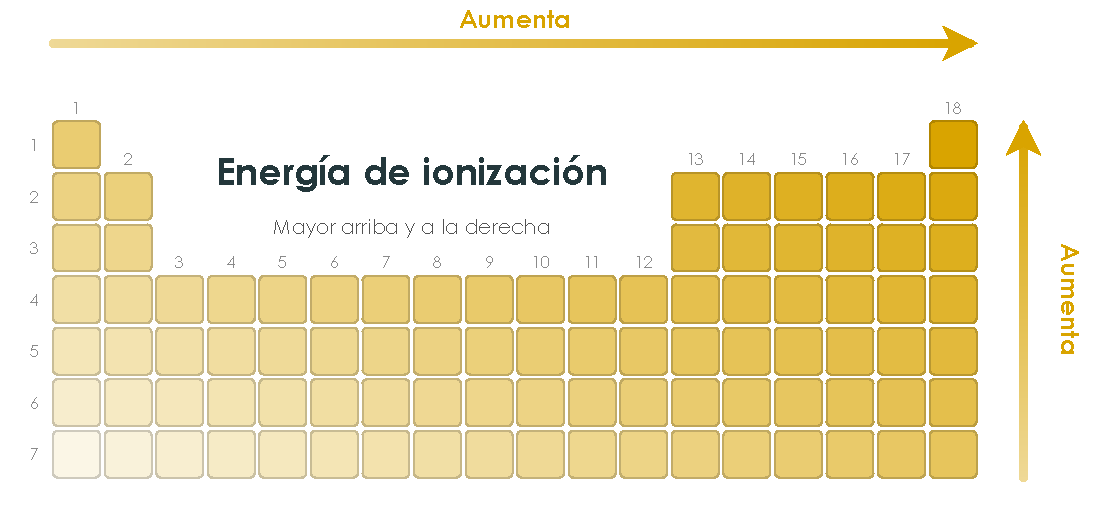
\includegraphics[width=0.85\linewidth]{FigurasSVG/UD2_Tabla_Periodica/pdf/UD2_04_variacion_energia_ionizacion.pdf}
    \caption{Variación de la EI}
    \label{fig:variacionei}
\end{figure}

A continuación, tenemos una tabla con los valores de EI. Como podemos apreciar, existe una anomalía entre la EI del \ch{Be} y el \ch{B}, que se debe a que el \ch{Be} tiene su capa de valencia llena y, por tanto, su tendencia a perder electrones es menor que en el caso del boro, que tiene un electrón en el orbital \( p \).
Algo similar ocurre entre el nitrógeno y el oxígeno.

\begin{table}[H]
    \centering
    \caption{Variación de la energía de ionización}
    \vspace*{-8pt}
    % --- tabla antigua ---
    % \begin{tblr}{|c|c|c|c|c|c|c|c|c|}
        % \hline
        % \SetColumn{mybluecolour} \textbf{\textcolor{white}{Elemento}} & \textbf{\ch{Li}} & \textbf{\ch{Be}} & \textbf{\ch{B}} & \textbf{\ch{C}} & \textbf{\ch{N}} & \textbf{\ch{O}} & \textbf{\ch{F}} & \textbf{\ch{Ne}}   \\
        % \hline
        % \textbf{\textcolor{white}{Valor (eV)}}:                       & 5.38             & 9.25             & 8.26            & 11.22           & 14.48           & 13.65           & 17.34           & 21.45            \\
        % \hline
    % \end{tblr}
    % --- tabla nueva ---
    \begin{tabular}{@{}ccccccccc@{}}
        \toprule
        \SetColumn{mybluecolour} \textbf{\textcolor{white}{Elemento}} & \textbf{\ch{Li}} & \textbf{\ch{Be}} & \textbf{\ch{B}} & \textbf{\ch{C}} & \textbf{\ch{N}} & \textbf{\ch{O}} & \textbf{\ch{F}} & \textbf{\ch{Ne}} \\[3pt]
        \textbf{\textcolor{white}{Valor (eV)}}: & 5.38 & 9.25 & 8.26 & 11.22 & 14.48 & 13.65 & 17.34 & 21.45 \\
        \bottomrule
    \end{tabular}
\end{table}
% \begin{figure}[H]
%     \centering
%     \includegraphics[scale=1]{images/UD2/ei1.png}
%     \caption{Variación EI}
%     \label{fig:variacionei2}
% \end{figure}
\begin{table}[H]
    \centering
    \caption{Configuración electrónica del Be, N, B y O}
    \vspace*{-8pt}
    % --- tabla antigua ---
    % \begin{tblr}[caption = {Configuración electrónica},]{|c|c|}
        % \hline
        % \textbf{\ch{Be}}: \elconf{Be} & \textbf{\ch{N}}: \elconf{N} \\
        % \hline
        % \textbf{\ch{B}}: \elconf{B}   & \textbf{\ch{O}}: \elconf{O} \\
        % \hline
    % \end{tblr}
    % --- tabla nueva ---
    \begin{tabular}{@{}cc@{}}
        \toprule
        \textbf{\ch{Be}}: \elconf{Be} & \textbf{\ch{N}}: \elconf{N} \\[3pt]
        \textbf{\ch{B}}: \elconf{B} & \textbf{\ch{O}}: \elconf{O} \\
        \bottomrule
    \end{tabular}
\end{table}
% \begin{figure}[H]
%     \centering
%     \includegraphics[scale=1]{images/UD2/ei2.png}
%     \caption{Configuración electrónica}
%     \label{fig:configuracionele}
% \end{figure}
\begin{consejo}[Analizar la tendencia del Radio y PI/EI]
    \begin{enumerate}
        \item Estas dos propiedades siempre se analizan teniendo en cuenta la carga nuclear y/o la carga nuclear efectiva.
        \item Cuando analicemos los elementos que están en un mismo período, se utilizará la \textbf{carga nuclear} como referencia, puesto que todos esos elementos tienen el mismo nivel energético con electrones y, por tanto, no tiene sentido hablar de apantallamiento (\(\sigma\)). En este caso debemos decir que, al aumentar el número atómico, aumentará la carga nuclear, quedando, en consecuencia, los electrones más atraídos por el núcleo.
        \item En el caso de que estemos analizando elementos del mismo grupo, hay que justificar su tendencia utilizando la carga nuclear efectiva, \(Z_{eff}\), ya que en este caso, al bajar en el grupo vamos aumentando los niveles energéticos, lo que aumenta el número de electrones y, por tanto, el apantallamiento será mayor (repulsión entre electrones).
        Cuando bajamos en un grupo, aumenta el apantallamiento, disminuyendo así la carga nuclear efectiva (recordamos que \(Z_{eff} = Z - \sigma\)).
    \end{enumerate}
\end{consejo}


\begin{example}
    Dados los elementos K (Z=19), Ca (Z=20), Zn (Z=30), F (Z=9) y Ne (Z=10), ordénalos razonadamente, de menor a mayor, de acuerdo con sus valores de: a) radio atómico; b) energía de ionización.

        {\negsubro{Solución:}}

    Lo primero que debemos hacer es situar el grupo y el período de cada elemento. Ayuda mucho poner la configuración de su capa de valencia, es decir, la configuración electrónica del último nivel ocupado.
    \begin{itemize}
        \item \ch{K}: \elconf{K}
        \item \ch{Ca}: \elconf{Ca}
        \item \ch{Zn}: \elconf{Zn}
        \item \ch{F}: \elconf{F}
        \item \ch{Ne}: \elconf{Ne}
    \end{itemize}

    \begin{enumerate}[label=\letraminuscula]
            \item Ordenación según el radio atómico.

            Aquí tenemos uno de los casos más complejos en los que nos podemos encontrar. Tenemos tres elementos que están en el período 4 (K, Ca y Zn) y otros elementos que están en el período 2 (F y Ne).
            Sabemos que al bajar en la tabla periódica, aumenta la carga nuclear, pero también aumenta el apantallamiento (más electrones que provocan repulsiones), provocando que la carga nuclear efectiva sea menor \( Z_{eff} = Z - \sigma \).
            Si disminuye la carga nuclear efectiva, los electrones estarán menos atraídos por el núcleo y, por tanto, su radio atómico aumentará.
            Llegados a este punto, podemos decir que los elementos K, Ca y Zn tendrán un radio atómico mayor que los elementos F y Ne.
            Los que tendrán menor radio serán el \ch{F} y el \ch{Ne}.
            Ambos están en el mismo período y, por tanto, no tiene sentido hablar de apantallamiento.
            Al tener el \ch{Ne} mayor número atómico, tendrá una mayor carga nuclear y, por tanto, los electrones estarán más atraídos por el núcleo, lo que hará que tenga un radio atómico menor que el del \ch{F}.
            Por lo tanto, \( \ch{Ne} < \ch{F} \).

            Ahora ordenemos los elementos \ch{K}, \ch{Ca} y \ch{Zn}.
            Estos también están todos en el mismo período. El de menor radio será el \ch{Zn}, ya que tiene una mayor carga nuclear, seguido del \ch{Ca} y finalmente el \ch{K}.

            Finalmente, la ordenación por radio atómico quedará de la siguiente manera:
            \[
                \ch{Ne} < \ch{F} < \ch{Zn} < \ch{Ca} < \ch{K}
            \]
            \item Ordenación de la energía de ionización.

            El grupo de los elementos \ch{K}, \ch{Ca} y \ch{Zn} tendrá una energía de ionización menor que los del grupo \ch{F} y \ch{Ne}, ya que los primeros tienen una carga nuclear efectiva menor que los otros y, por tanto, los electrones están menos atraídos por el núcleo, lo que facilita la extracción de un electrón, necesitándose así menor energía (menor energía de ionización).

            Vamos a ordenar primero este grupo.
            Al estar los tres en el mismo período, \ch{K} será el que tenga menor energía de ionización, ya que su carga nuclear es menor y, por tanto, los electrones estarán menos atraídos por el núcleo, luego le sigue el \ch{Ca} y luego el \ch{Zn}.
            Quedando este grupo como \( \ch{K} < \ch{Ca} < \ch{Zn} \).

            Ahora pasamos al grupo del \ch{F} y el \ch{Ne}.
            El \ch{Ne} tiene mayor carga nuclear, lo que incrementa la atracción de los electrones y, por tanto, una mayor energía de ionización (\( \ch{F} < \ch{Ne} \)).

            El resultado final quedará, por tanto, como:
            \begin{equation*}
                \ch{K} < \ch{Ca} < \ch{Zn} < \ch{F} < \ch{Ne}
            \end{equation*}
    \end{enumerate}
\end{example}

\subsection{Afinidad electrónica (AE)}

\begin{definition}[Afinidad electrónica (AE)]
        Es la energía involucrada cuando un átomo en estado gaseoso capta un electrón, formándose un ion negativo.
        \begin{centeredequation}
           X(g) + e^- \longrightarrow X^- (g)
        \end{centeredequation}
        Se mide en unidades de energía: \unit{\kilo\joule\per\mole}, \unit{\joule\per \text{átomo}}, \unit{\electronvolt\per \text{átomo}}.
\end{definition}

El signo negativo de estas AE indica que se trata de una energía desprendida cuando el átomo capta un electrón.
Los elementos con AE positivas no muestran tendencia a captar electrones.

También se puede dar el caso de una segunda o tercera AE, estos casos son difíciles de calcular y no tienen una variación regular.

\begin{enumerate}[label=\numberballmDarkTeal]
        \item En un grupo como en un período, al aumentar la carga nuclear se eleva la atracción electrostática del núcleo sobre el electrón y se libera más energía, es decir, la AE es mayor.
        \item Al descender en un grupo, se intensifica el \textbf{efecto pantalla}, provocando así una disminución de la carga nuclear efectiva, liberándose menor energía al capturar el electrón, lo que provoca una disminución de la AE.
        \item Al aumentar la capa de valencia, el electrón que se capta estará más alejado del núcleo, experimentando una menor atracción y, por tanto, una menor AE.
\end{enumerate}
% \begin{enumerate}[label=\numberballmDarkTeal]
%     \item \negrita{Grupo}: En un grupo, el valor de la AE disminuye al bajar en el grupo. En la siguiente table se muestra un valor anómalo para el \ch{F} debido a que este es más pequeño y la adición de un electrón provoca un aumento en la repulsión. Los valores están dados en valores absolutos.
%     \begin{figure}[H]
%         \centering
%         \includegraphics[scale=1]{aetabla.png}
%         \caption{Valores de AE}
%         \label{fig:valoresddeae}
%     \end{figure}
%     \item \negrita{Periodo}: aumenta de izquierda a derecha
% \end{enumerate}
Podemos decir que la AE aumenta al subir en un grupo y al desplazarse a la derecha en un período, a excepción de los gases nobles, es decir, es mayor cuanto más arriba y más a la derecha de la tabla periódica.
\begin{figure}[H]
    \centering
    % [FIGURA ORIGINAL] \includegraphics[scale=0.2]{images/imagesUD2TablaPeriodica/UD2_Teoria/variacionae2.png}
    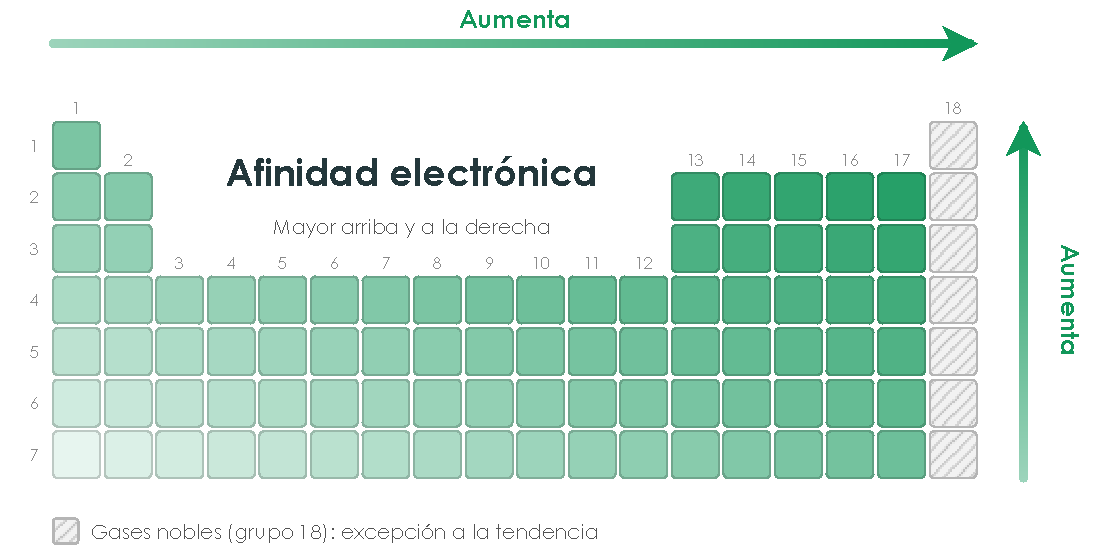
\includegraphics[width=0.85\linewidth]{FigurasSVG/UD2_Tabla_Periodica/pdf/UD2_05_variacion_afinidad_electronica.pdf}
    \caption{Variación de la AE}
    \label{fig:variacionae}
\end{figure}

\subsection{Electronegatividad}

    \begin{definition}[Electronegatividad (EN)]
        Es la tendencia que tiene un átomo a atraer hacia sí los electrones de un enlace químico.
        Se puede expresar en unidades de energía como \unit{\kilo\joule\per\mole}, pero es habitual expresarlo en una escala arbitraria que da una idea cualitativa de esa tendencia.
    \end{definition}

Es muy importante no confundir la electronegatividad con la afinidad electrónica.
Debemos tener en cuenta que la electronegatividad se debe a la tendencia de un átomo a llevarse los electrones cuando están formando un enlace mientras que la afinidad electrónica es la tendencia que tiene un átomo a ganar un electrón.

\begin{enumerate}[label=\numberballmDarkTeal]
        \item \negrita{Grupo}: disminuye a medida que aumenta el número atómico.
        \item \negrita{Periodo}: aumenta de izquierda a derecha.
\end{enumerate}

La \textbf{electronegatividad} aumenta al subir en un grupo y al desplazarse a la derecha en un período, a excepción de los gases nobles, es decir, es mayor cuanto más arriba y a la derecha de la tabla periódica se encuentre el elemento químico.
\begin{figure}[H]
    \centering
    % [FIGURA ORIGINAL] \includegraphics[scale=0.2]{images/imagesUD2TablaPeriodica/UD2_Teoria/variacionelectronegatividad2.png}
    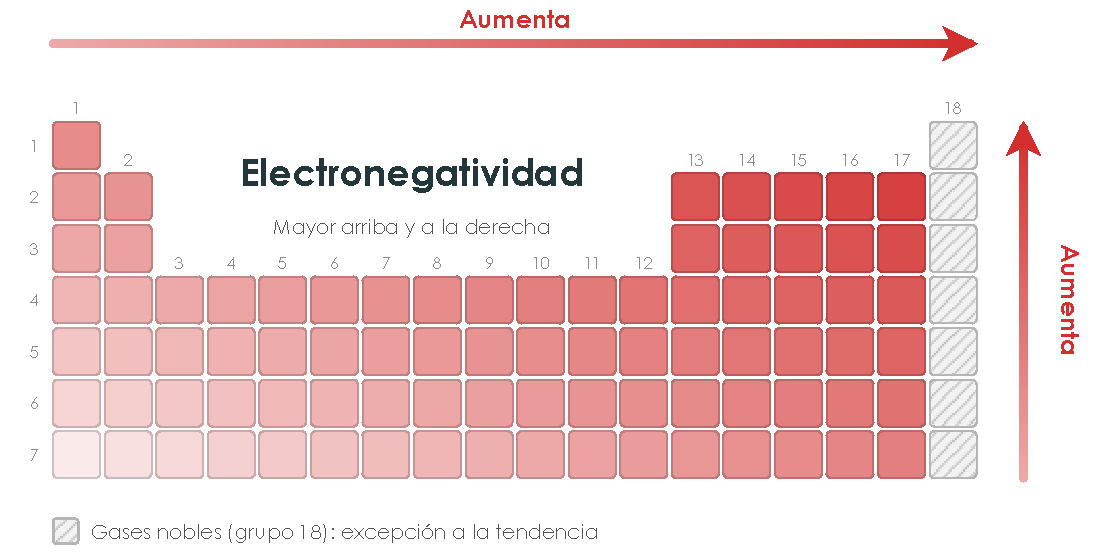
\includegraphics[width=0.85\linewidth]{FigurasSVG/UD2_Tabla_Periodica/pdf/UD2_06_variacion_electronegatividad.pdf}
    \caption{Variación de la electronegatividad}
    \label{fig:variacionelectronegatividad}
\end{figure}

Los valores de la electronegatividad se pueden obtener según la expresión:
\begin{centeredequation}
     \text{Electronegatividad} = \dfrac{EI + AE}{2}
\end{centeredequation}
A modo informativo, en la figura \ref{fig:tabla de electronegatividades de Pauling} tenemos una tabla con el valor de las electronegatividades de los elementos.

\begin{figure}[H]
    \centering
    % [FIGURA ORIGINAL] \includegraphics[scale=.3]{images/imagesUD2TablaPeriodica/UD2_Teoria/pauling electronegativity table_b.png}
    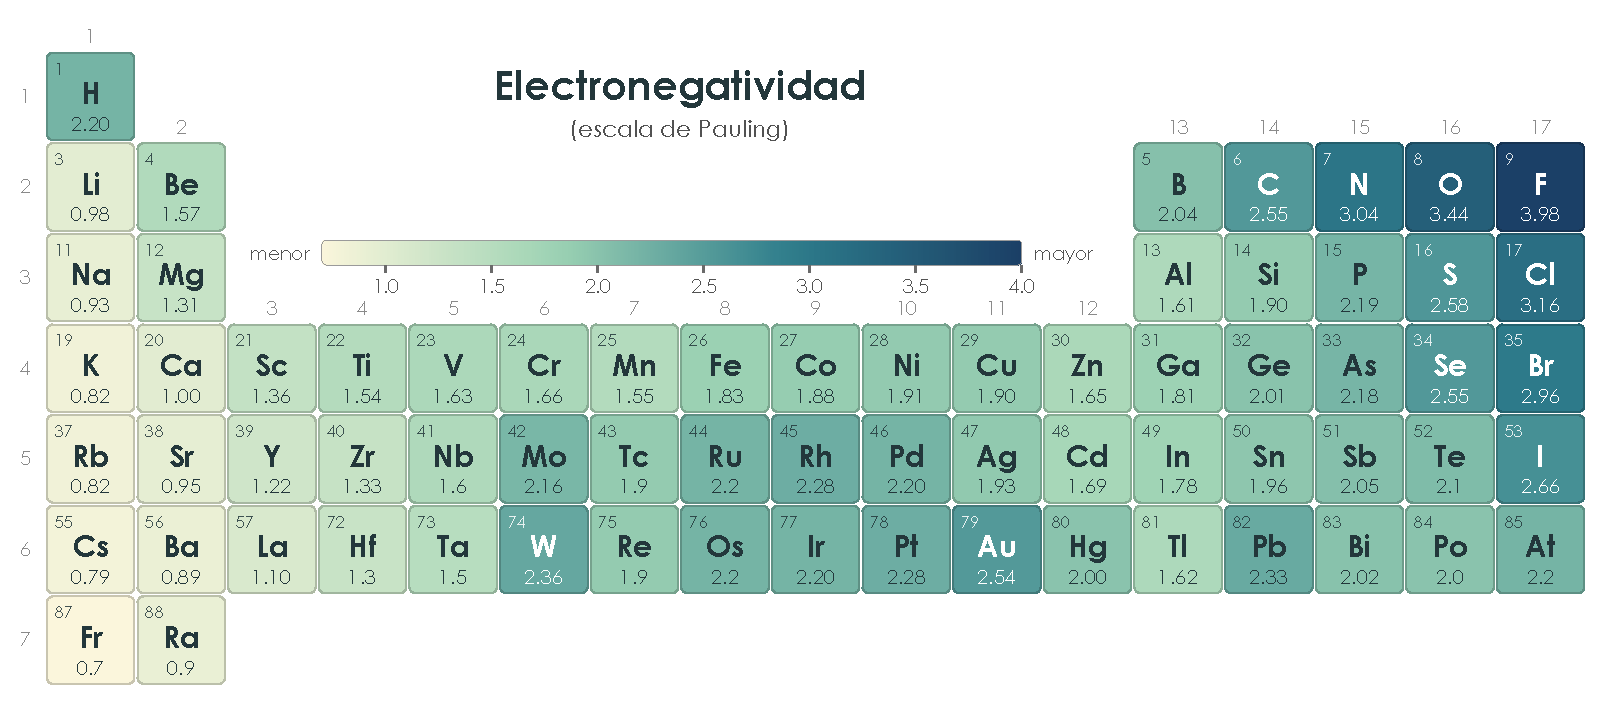
\includegraphics[width=1.0\linewidth]{FigurasSVG/UD2_Tabla_Periodica/pdf/UD2_07_tabla_electronegatividades_pauling.pdf}
    \caption{Tabla de electronegatividades de Pauling}
    \label{fig:tabla de electronegatividades de Pauling}
\end{figure}

\subsection{Otras propiedades químicas y físicas}

\begin{enumerate}[label=\numberballmDarkTeal]
        \item \negsubro{Número de oxidación}. Es una consecuencia directa de la configuración electrónica y, por lo tanto, de la situación de un elemento en la TP.
        \item \negsubro{Carácter metálico}. El carácter metálico lo podemos definir a partir de la electronegatividad.
        Los elementos metálicos tienen tendencia a ceder electrones.
        Los elementos con bajos potenciales de ionización y bajas afinidades electrónicas tendrán más carácter metálico.
\end{enumerate}


